%% ma: L12-B01-0009
%% lop: 12
%% chuong: 1
%% bai: 1
%% dang: 12.1.3
%% loai: TN4
%% muc: TH
%% dap_an: "C"
%% nguon: "(NBV)-ĐỀ SỐ 6-MỖI NGÀY 1 ĐỀ THI 2025.pdf (D06, MỖI NGÀY 1 ĐỀ - Đề số 6), Phần I Câu 6"
%% kien_thuc: "Bài 1 (đọc điểm cực đại từ bảng xét dấu của đạo hàm)"
%% trang_thai: chinh-thuc
%% ghi_chu: "Trùng ý tưởng với dạng 12.1.3 (đọc bảng biến thiên, giáo viên đã duyệt gộp các câu đọc cực trị) nên nhập cùng dạng; ở đây cho bảng xét dấu của f'(x). Đáp án gốc C đúng"
\begin{ex}
Cho hàm số $y=f(x)$ liên tục trên $\mathbb R$ và có bảng xét dấu của đạo hàm như sau:
\begin{center}
\begin{tikzpicture}
  \tkzTabInit[lgt=1.5,espcl=2.2]{$x$/.8,$f'(x)$/.8}{$-\infty$,$-2$,$0$,$2$,$+\infty$}
  \tkzTabLine{,+,0,-,0,+,0,-,}
\end{tikzpicture}
\end{center}
Số điểm cực đại của hàm số đã cho là
\choice{$0$}{$1$}{\True $2$}{$3$}
\loigiai{$f'(x)$ đổi dấu từ $+$ sang $-$ khi qua $x=-2$ và $x=2$ nên hàm số đạt cực đại tại hai điểm này; tại $x=0$ đạo hàm đổi dấu từ $-$ sang $+$ nên là điểm cực tiểu. Vậy hàm số có $2$ điểm cực đại.}
\end{ex}
